\subsection{Components of CNN}
There are \tB{neural networks using \emph{convolution}} operation instead of general 
matrix multiplication \uB{in at least on of their layers}.
\begin{enumerate}
    \item Apply several convolution in parallel to produce a set of activation 
        functions
    \item The previous activation functions are run through nonlinear activation 
        function (\emph{detector stage})
    \item Modify the output of the layer further with \textbf{pooling functions}
\end{enumerate}

\paragraph{Convolution}
\subparagraph{Convolution operation} \tB{allows to reduce the noise coming from
observation by considering multiple observations and averaging them}. However we want 
to have the \uB{ability to give more weight to some observations}, the more recent ones
for example.
Let's assume we observe \tB{a signal $x(t)$} (\emph{input}) and we have a \tB{weighting
function $w(a) $}(\emph{kernel}) where \uB{$a$ is the age of a measurement} the
resulting signal issued from convolution (\emph{feature map}) is:
\begin{center}
    \tR{$s(t) = (x * w)(t) = \Su{}{}x(a)w(t-a)da$}\\
    or in matrix convention\\
    $\bm{S}(n,p) = \left(\bm{I}*\bm{K}\right)(n, p) = \su{i}{}\su{j}{}\bm{I}(i, j)
    \bm{K}(n-i, p-j) = \su{i}{}\su{j}{}\bm{I}(n-i, p-j) \bm{K}(i, j) =
    \left(\bm{K}*\bm{I}\right)(n, p)$ 
\end{center}
\begin{figure}[H]
    \begin{center}
        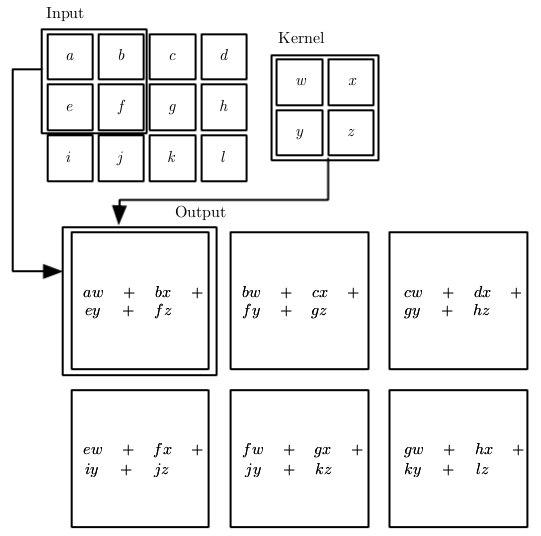
\includegraphics[width=.5\textwidth]{./chapters/4_deep_learning/3_types_of_neural_networks/images/01_convolutional_graph.png}
    \end{center}
    \caption{2-D convolution without kernel-flipping}
    \label{fig:01_convolutional_graph}
\end{figure}

\subparagraph{Motivation}
\begin{itemize}
    \item \textbf{sparse interactions} (due to reduced size of kernel compare with the 
        input one)
    \item \textbf{parameter sharing} (rather than learning a separate set of 
        parameters, for every location we learn only one set, that are the kernel's 
        ones)
    \item \textbf{equi-variant representations}: \tG{$f(x)$ is equi-variant to a
            function $g$ if $f\left(g(x)\right) = g\left(f(x)\right)$}. For example 
            \uB{if $g$ is any function that translates the input then the convolution 
            is equi-variant to $g$}
        \begin{itemize}
            \item for time series, \tB{convolution produces a sort of timeline showing
                when different features appear in the input}.\\
                By moving an event later in time in the input will induce that the same
                representation of the event will appear in the output
            \item for images, \tB{convolution creates a 2-D map of where certain 
                features appear in the input}.\\
                By moving the object in the input, its representation will move the 
                same amount in the output
        \end{itemize}
    \item \textbf{ability to work with inputs of variable size}
\end{itemize}


\paragraph{Pooling}
\subparagraph{Purpose} of pooling is to \tB{make representation become approximately
\emph{invariant} to small translations of the input}. Such a priority can be very
useful when we are searching for the presence of some feature rather than their 
location.\\
It can be viewed as \uB{adding an infinitely strong prior to the weight resulting in 
layer invariance} to small translations

\subparagraph{Examples of pooling}
\begin{figure}[H]
    \begin{center}
        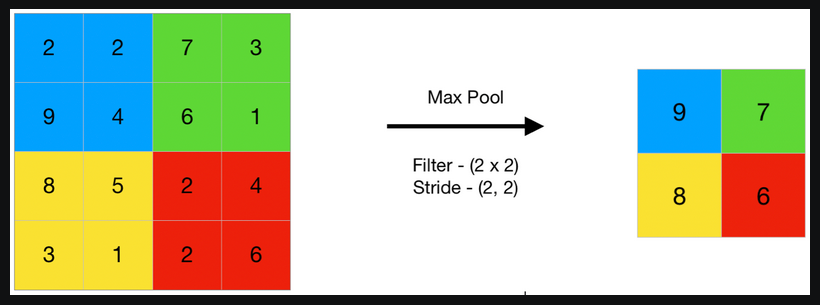
\includegraphics[width=.5\textwidth]{./chapters/4_deep_learning/3_types_of_neural_networks/images/02_pooling_max.png}
    \end{center}
    \caption{Max pooling}
    \label{fig:02_pooling_max}
\end{figure}


\begin{figure}[H]
    \begin{center}
        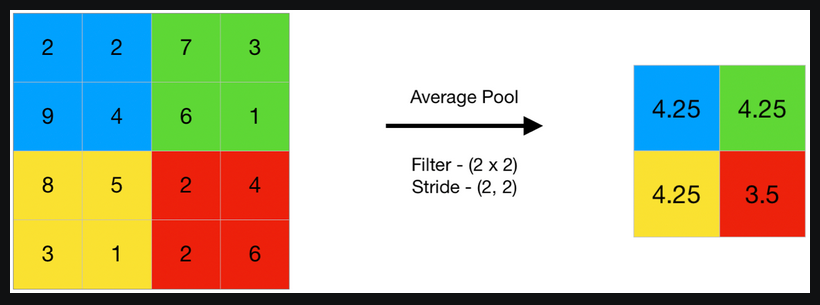
\includegraphics[width=.5\textwidth]{./chapters/4_deep_learning/3_types_of_neural_networks/images/02_pooling_average.png}
    \end{center}
    \caption{Max pooling}
    \label{fig:02_pooling_average}
\end{figure}
